\chapter{Lake Macalania}

\begin{enumerate}
    \item Run up and \sd
\end{enumerate}
\begin{battle}[16000]{Crawler}
    \begin{itemize}
        \switch{\tidus}{\rikku}
        \rikkuf Lightning Marble x1/2 Negator (1\,000 HP)
        \rikkuf Lightning Marble Crawler
        \kimahrif Lightning Marble Crawler
        \luluf Phoenix Down \rikku
        \rikkuf Lightning Marble Crawler
        \ifthenelse{\equal{\blitzresult}{win}}{%
            \switch{\lulu}{\yuna}
            \yunaf Mega Phoenix
            \switch{\yuna}{\tidus}
            \tidusf Equip Brotherhood
        }{\ifthenelse{\equal{\blitzresult}{loss}}{%
            \kimahrif If you need a Lunar Curtain Steal Crawler, else Defend
            \switch{\lulu}{\yuna}
            \yunaf If 2 Characters dead Mega Phoenix, else Phoenix Down \rikku
            \switch{\yuna}{\tidus}
            \tidusf If \kimahri\ is dead Phoenix Down him, otherwise Equip Brotherhood
        }{%
            \kimahrif If \blitzloss\ and you need a Lunar Curtain Steal Crawler, else Defend
            \switch{\lulu}{\yuna}
            \yunaf If 2 Characters dead Mega Phoenix, else Phoenix Down \rikku
            \switch{\yuna}{\tidus}
            \tidusf If \kimahri\ is dead Phoenix Down him, otherwise Equip Brotherhood
        }}
        \rikkuf \od\ Lv. 2 Key Sphere and Lightning Marble
    \end{itemize}
    \tidus, \yuna, \lulu\ and \kimahri\ need AP.
\end{battle}
\bothvfill
\winvfill
\lossvfill
\begin{spheregrid}
    \begin{itemize}
        \kimahrif (12 S.Lvl)
        \begin{itemize}
            \item Move $\downarrow\downarrow\downarrow\downarrow$ on the Luck node
            \item HP +200, Agi+4
        \end{itemize}
        \ifthenelse{\equal{\colstyle}{multi}}{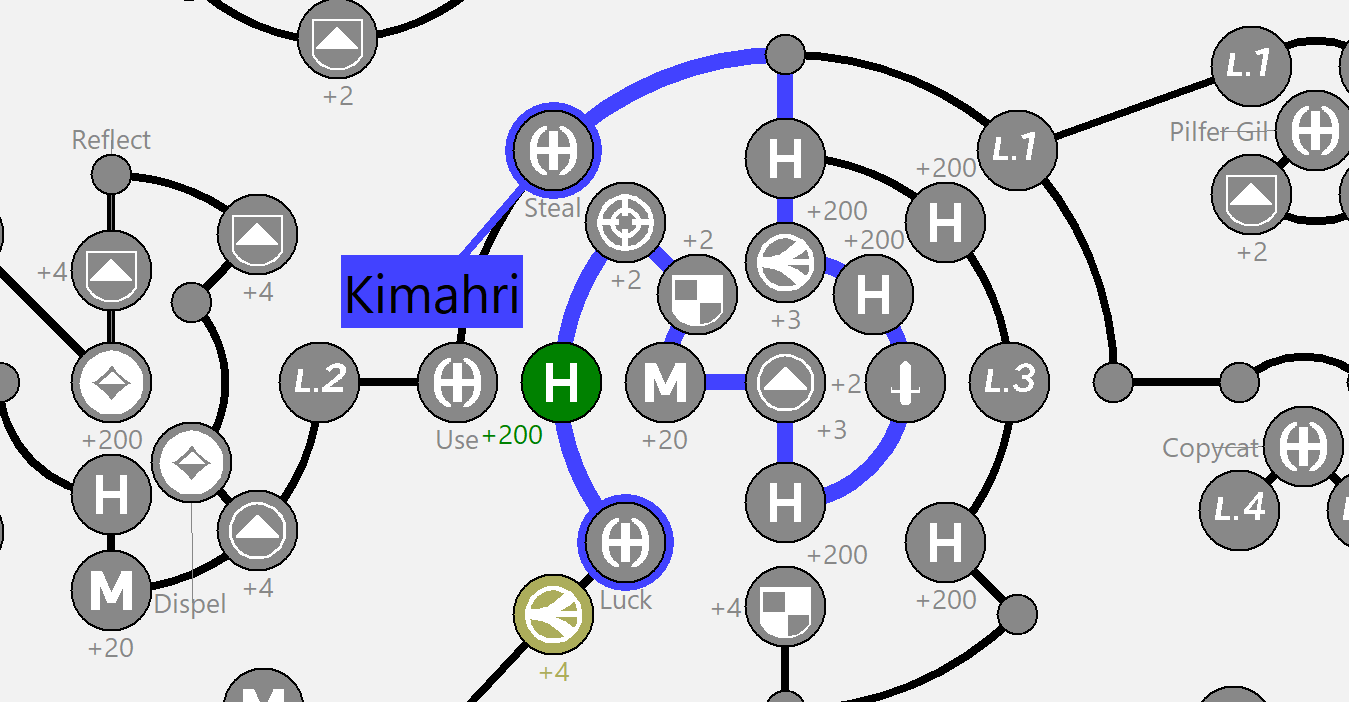
\includegraphics[width=.8\columnwidth]{graphics/macalania_kimahri}}{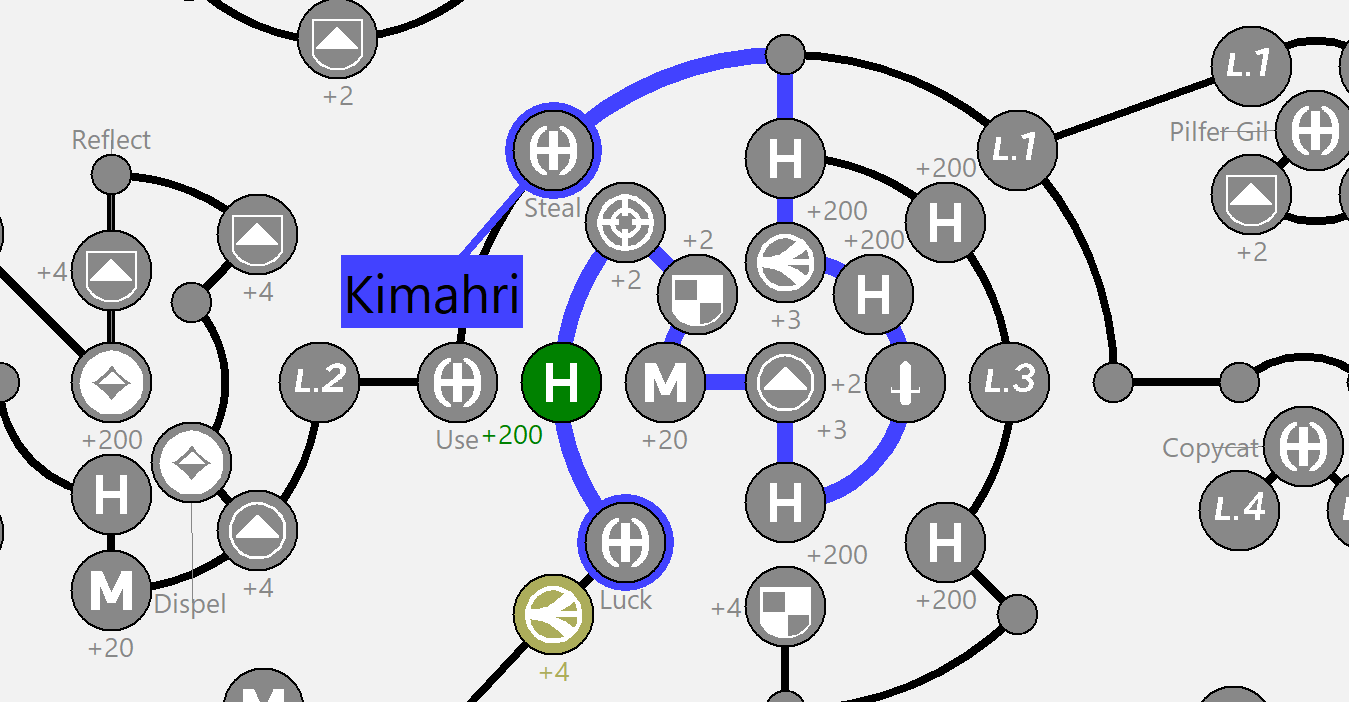
\includegraphics[width=.5\columnwidth]{graphics/macalania_kimahri}}
        \tidusf (22 S.Lvl)
        \begin{itemize}
            \item Level 2 Key Sphere
            \item Move $\rightarrow\uparrow$
            \item Str +4
            \item Move $\uparrow\uparrow$
            \item HP+200
            \item Move $\rightarrow\rightarrow\uparrow$
            \item HP+200, Str+4, Agi+2
            \blitzballdetermination[true]{%
                \item Move $\rightarrow$
                \item Use Strength Sphere, Activate it
                \item Move $\uparrow\leftarrow\leftarrow$ or $\nwarrow\nwarrow$
            }{%
                \item Move $\uparrow\nwarrow$
            }
            \item HP+200, Str+4, Agi+2
            \item Move $\leftarrow$
            \item Str+4
        \end{itemize}
        \ifthenelse{\equal{\colstyle}{multi}}{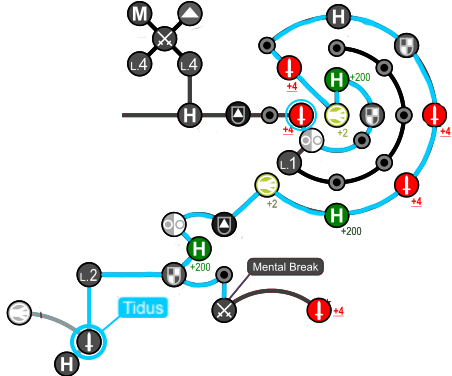
\includegraphics[width=.8\columnwidth]{graphics/Tidus_post_crawler}}{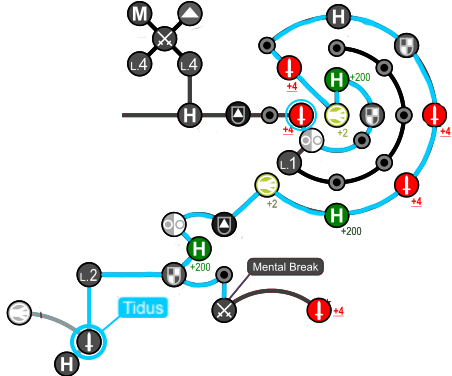
\includegraphics[width=.5\columnwidth]{graphics/Tidus_post_crawler}}
    \end{itemize}
\end{spheregrid}
\begin{enumerate}[resume]
    \item \sd, \cs[0:40], head to next screen
    \item Head to Temple, \sd. \save.
    \wincb
    \item Jyscal Skip (Ignore if playing with Cutscene Remover):
    \begin{itemize}
        \item Speak to Tromell for \textbf{Shell Targe}
        \item Walk into the wall to the right of Tromell
        \item Move slightly to the right, turn around and Talk to Tromell while moving Right.
        \item If successful, walk forward while mashing Shelinda's dialogue.
        \item When dialogue finishes, walk up the stairs, push the man, and go through.
        \item If Shelinda is not saying her dialogue, talk to one of the musicians
    \end{itemize}
    \item \sd, walk to Fayth room, \cs[2:10]
\end{enumerate}
\bothvfill
\begin{battle}[3000]{Seymour}
    \begin{itemize}
        \tidusf Haste \tidus
        \yunaf Change Weapon to Staff
        \kimahrif \od\ Stone Breath
        \tidusf Talk to Seymour
        \switch{\yuna}{\auron}
        \auronf Defend
        \enemyf Seymour Blizzara
        \ifthenelse{\equal{\blitzresult}{win}}{%
            \tidusf Defend
        }{\ifthenelse{\equal{\blitzresult}{loss}}{%
            \tidusf Cheer
        }{%
            \tidusf if \blitzloss\ Cheer, else Defend
        }}
        \tidusf Attack
    \end{itemize}
\end{battle}
\bothvfill
\lossvfill
\begin{battle}[18000]{Anima}
    \begin{itemize}
        \blitzballdetermination[true]{%
            \kimahrif Defend
            \auronf Defend
            \switch{\tidus}{\wakka}
            \wakkaf Change Weapon to anything
            \enemyf Pain
            \switch{first survivor}{\tidus}
            \tidusf Attack x4
            \switch{second survivor}{\rikku}
            \rikkuf Steal x2
        }{%
            \kimahrif Lightning Marble Anima
            \switch{\auron}{\rikku}
            \rikkuf Lightning Marble Anima
            \switch{\tidus}{\wakka}
            \wakkaf Change Weapon to anything
            \enemyf Pain
            \switch{first survivor}{\tidus}
            \tidusf Attack x4
            \switch{second survivor}{\rikku\ or \kimahri}
            \item \rikku\ or \kimahri: Steal
        }
        \item \textit{If Tidus Misses:}
        \begin{itemize}
            \item On Tidus' 4th turn switch him for \lulu
            \luluf Phoenix Down dead character
            \enemyf Pain
            \switch{first survivor}{\tidus}
            \item Continue the fight like normal
        \end{itemize}
    \end{itemize}
\end{battle}
\begin{battle}[6000]{Seymour}
    \begin{itemize}
        \blitzballdetermination[true]{%
            \tidusf Phoenix Down \rikku\ if she died before Multi-Thundara, otherwise Change Weapon to Sonic Steel, then Defend x2 until Multi-Thundara.
        }{%
            \tidusf Phoenix Down \rikku\ if she died before Multi-Thundara, otherwise Defend x2 until Multi-Thundara.
        }
        \rikkuf Defend
        \tidusf Attack x2
    \end{itemize}
    \tidus\ and \yuna\ need AP.
\end{battle}
\begin{enumerate}[resume]
    \item Name \shiva
\end{enumerate}
\begin{spheregrid}
    \begin{itemize}
        \tidusf
        \begin{itemize}
            \item Move $\leftarrow\leftarrow\leftarrow\leftarrow$
            \item HP+200, Str+4
            \item Move $\leftarrow$
            \item Agi+2
        \end{itemize}
        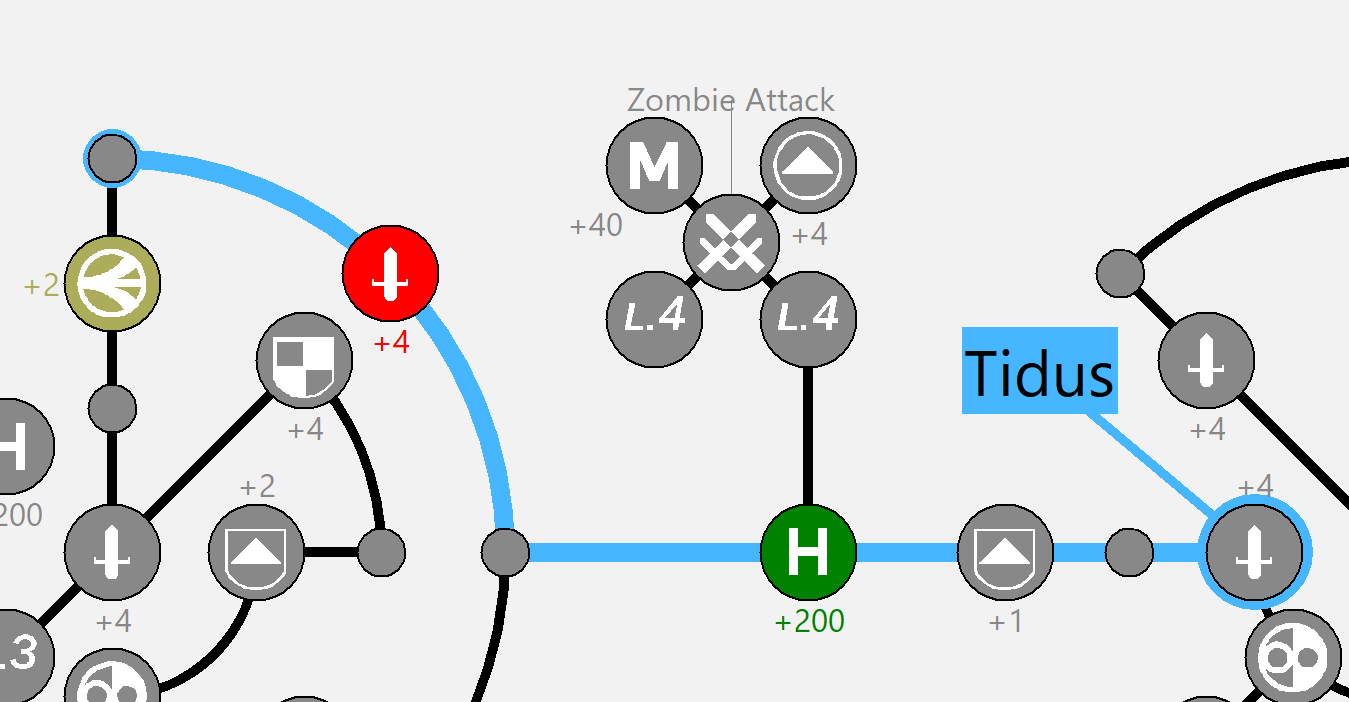
\includegraphics[width=.8\columnwidth]{graphics/Tidus_Post_Seymour}
    \end{itemize}
\end{spheregrid}
\winvfill
\begin{enumerate}[resume]
    \item You need 21 Power Spheres and 10 Speed Spheres \textbf{at this point} to be done farming them.
    \item \formation{\rikku}{\tidus}{\yuna}
    \ifthenelse{\equal{\blitzresult}{win}}{}{
        \ifthenelse{\equal{\blitzresult}{both}}{
            \item \textit{If you \lostblitz:}
        }{}
        \begin{equip}
            \begin{itemize}
                \tidusf Equip Sonic Steel
            \end{itemize}
        \end{equip}
    }
    \item \save, exit Fayth room. Make sure that the Save Sphere touch is done \textbf{after} the above Sphere Grid, otherwise you will die to Wendigo.
\end{enumerate}
\begin{trial}
    \begin{itemize}
        \item Slide pedestal to the right
        \item Take sphere from the right wall, place into pedestal
        \item Push pedestal up
        \item Take Glyph sphere from middle pillar
        \item Go downstairs and push pedestal to the right
        \item Place Glyph sphere in far left slot in the wall
        \item Go upstairs, pick up new sphere
        \item Go downstairs, place sphere in pillar
        \item Go upstairs, take the sphere at the top of the slope
        \item Place in last pillar
    \end{itemize}
\end{trial}
\begin{enumerate}[resume]
    \item Go to temple entrance, \sd
    \item Move south and go down the left path.
    \blitzballdetermination[true]{%
        \item Try to not get caught by the Guados chasing you, if you get caught Flee
    }{%
        \item Intentionally get caught by a Guado, kill the enemies to gain AP on Tidus
        \begin{encounters}
            \begin{itemize}
                \tidusf Attack Guado, then Surviving Enemies
                \rikkuf Silence Grenade
                \yunaf Defend
            \end{itemize}
        \end{encounters}
    }
\end{enumerate}
\blitzballdetermination{}{
\begin{spheregrid}
    \begin{itemize}
        \tidusf Move $\downarrow$
        \item Str+4
    \end{itemize}
    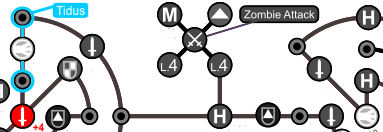
\includegraphics[width=.8\columnwidth]{graphics/tidus_bikanel}
\end{spheregrid}}
\winvfill
\bothvfill
\begin{battle}[18000]{Wendigo}
    \begin{itemize}
        \tidusf Haste \tidus
        \tidusf Switch Weapon to Brotherhood
        \tidusf Attack Guado B (Top One)
        \item \textit{If Light Curtain:}
        \begin{itemize}
            \rikkuf Light Curtain \tidus
        \end{itemize}
        \textit{Else:}
        \begin{itemize}
            \switch{\rikku}{\auron}
            \auronf Power Break
        \end{itemize}
        \tidusf Spiral Cut Wendigo, then Attack it until it's dead, then Attack Guado
        \yunaf Elixir \tidus/Phoenix Down dead character/Defend
        \switch{\yuna}{\lulu} on \yuna's 2nd turn
        \rikkuf Elixir \tidus/Phoenix Down dead character/Steal from the Guado/Defend
        \luluf Elixir \tidus/Phoenix Down dead character/Defend
    \end{itemize}
    \yuna, \tidus\ need AP. Helpful if \lulu\ gets it.
    Guaranteed 2 Power Spheres.
\end{battle}
\begin{enumerate}[resume]
    \item Run up to \rikku, \sd, walk up to \yuna, \sd, \save, run past \kimahri\ and go to the hidden area to \pickup{Level 2 Key Sphere}
    \winvfill
    \item Run up to \auron\ and speak with him, \sd, walk back, \cs+\skippablefmv[1:00], (press Start immediately after skip), \sd\ in Dream Sequence
\end{enumerate}